\chapter{Methods}
The main rule in this methodology is to keep the pipeline unchanged and modify only the training objective.
Each dataset is transformed into a uniform format.
Then, the model is loaded, QLoRA adapters are applied if needed, the model is trained with the chosen objective,
and evaluation is performed using the same generate-then-score protocol for every run.
Figure~\ref{Fig:Figure1} shows the full pipeline.

We intentionally keep the pipeline simple and controlled, because the goal is to isolate the effect of the training objective,
not to find the best possible score on each dataset.
Every experiment is defined through a configuration file that declares the dataset, the backbone, the objective, the adapter settings, the metrics, and the seed.
The same implementation is used for baseline evaluation, fine-tuning, and final evaluation, reducing the risk of hidden differences affecting the results.

\begin{figure}[!t]
\centering
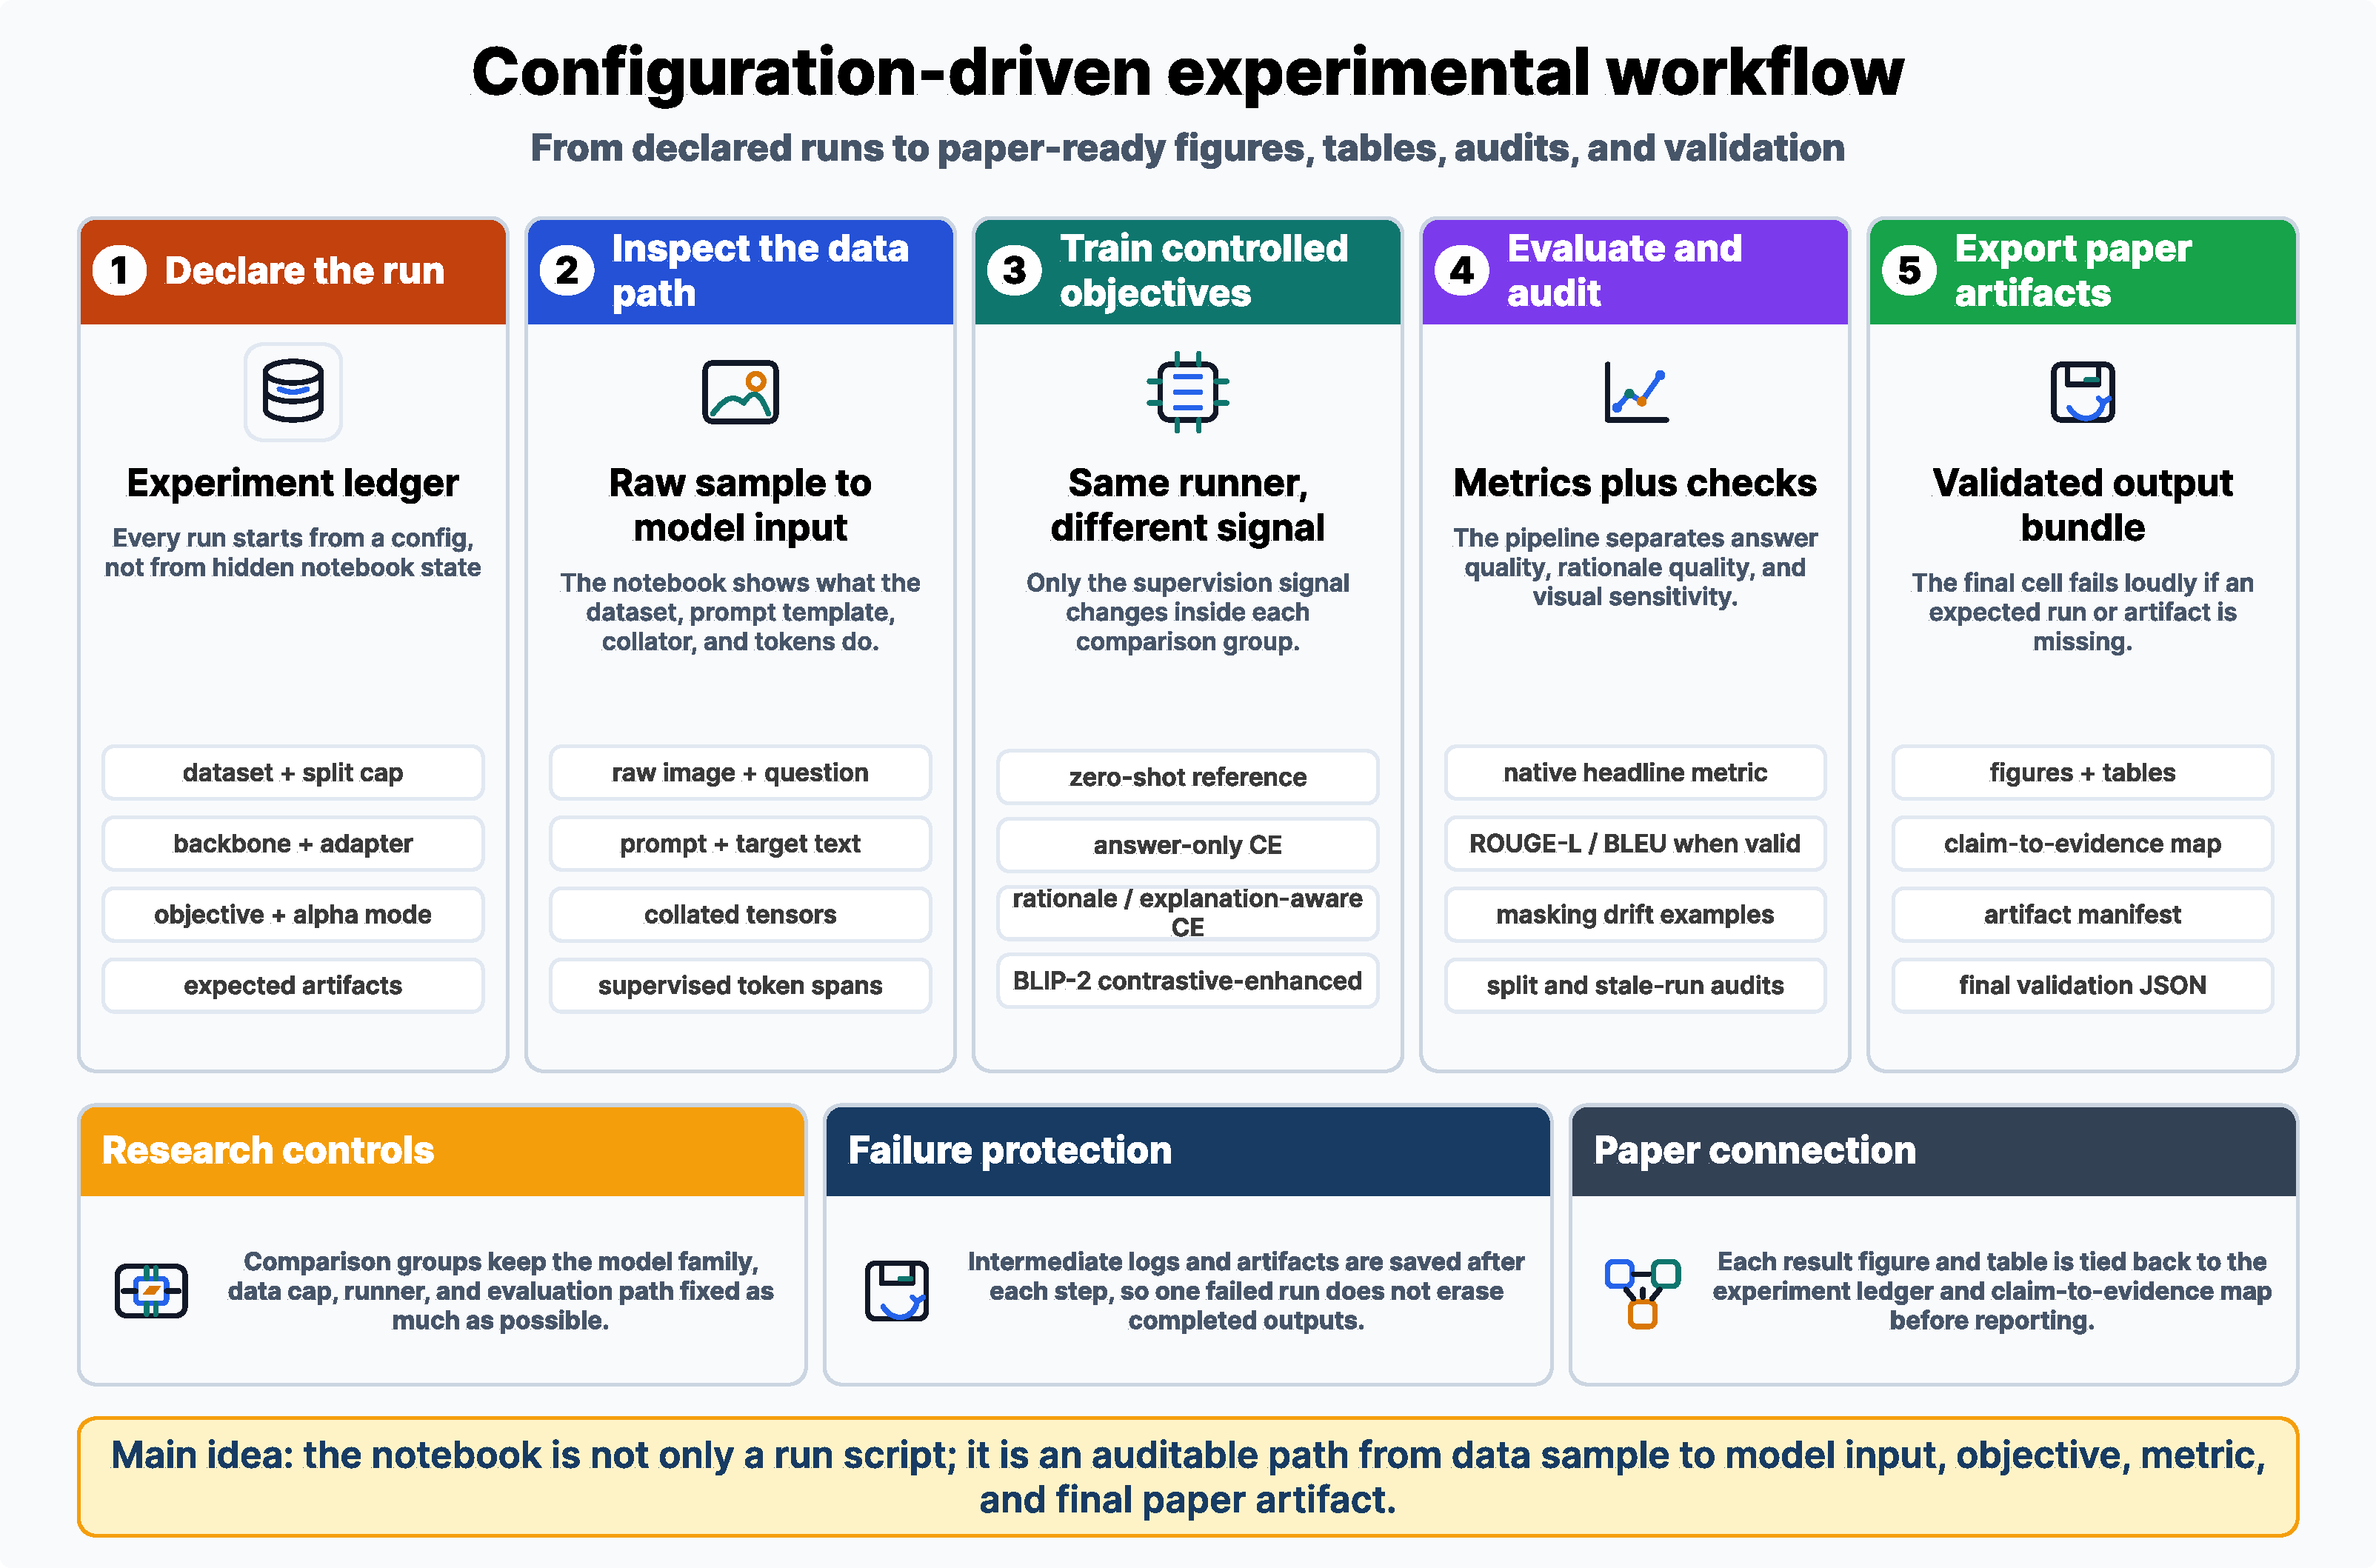
\includegraphics[width=1\linewidth]{./Figures/icons/Pipeline}
\caption{Configuration-driven experimental workflow.
Each run is declared through an experiment ledger, inspected through the data and prompt path, trained under the selected objective, evaluated with answer, rationale, and visual-sensitivity checks, and exported as paper-ready figures, tables, logs, and validation artifacts.}
\label{Fig:Figure1}
\end{figure}

\section{Datasets}
The experiments use five public datasets.
DocVQA represents document understanding, where the answer is usually based on scanned text, layout and local regions of the image~\cite{mathew2021docvqa}.
ChartQA is used for chart reasoning, in which the answer might depend on labels, axes, values, or relationships between elements in the chart~\cite{masry2022chartqa}.
ScienceQA provides multimodal science questions with multiple-choice answers and explanations, which is used for rationale supervision~\cite{lu2022scienceqa}.
A-OKVQA adds commonsense questions and rationales over natural images, which is also used for rationale-supervised training~\cite{schwenk2022aokvqa}.
VQAv2 is used as a general natural-image control, where the answer is often based on object recognition and simple relationships in the image~\cite{goyal2017vqav2}.
Table~\ref{tab:Datasets} summarises this dataset setup.

There is one important detail about the VQAv2 subset.
The experiment uses the configured \texttt{Erland/VQAv2-sample} source, which has 900 training examples and 100 evaluation examples.
Hence, we report it as a VQAv2 subset result, not as a full VQAv2 benchmark score.

All the datasets are transformed into a uniform format, where each example is comprised of an image, a question, an answer, and optionally a rationale.
If the dataset does not have gold rationales, the rationale field is left empty, and the training falls back to answer-only supervision.
Table~\ref{tab:InputConstruction} shows how these fields are turned into prompts and supervised targets.


\begin{table}[!ht]
\centering
\caption{Benchmarks used in the study. The sizes are rounded public benchmark sizes before filtering by image availability, answer type, or rationale availability. The completed experiments use capped train and evaluation splits so that every run fits the same practical compute budget.}
\label{tab:Datasets}
\begin{adjustbox}{max width=\textwidth}
\begin{tabular}{|l|l|c|l|c|l|}
\hline
\textbf{Dataset} & \textbf{Domain} & \textbf{Approx.\ size} & \textbf{Answer type} & \textbf{Gold rationale} & \textbf{Primary metric} \\ \hline
DocVQA~\cite{mathew2021docvqa} & Document & 50K & short text span & no & ANLS \\
ChartQA~\cite{masry2022chartqa} & Chart & 32K & numeric / short text & no & relaxed accuracy \\
ScienceQA~\cite{lu2022scienceqa} & Science image & 21K & multiple choice & yes & accuracy \\
A-OKVQA~\cite{schwenk2022aokvqa} & Commonsense image & 25K & multiple choice / short text & yes & accuracy \\
VQAv2 subset~\cite{goyal2017vqav2} & Natural image & 900/100 run split & open ended & no & VQA accuracy \\ \hline
\end{tabular}
\end{adjustbox}
\end{table}

\begin{table*}[!ht]
\centering
\caption{Input construction examples. The complete token, label, span, and collator traces are saved as pipeline artifacts; this table gives the paper-level view of what each prompt family means.}
\label{tab:InputConstruction}
\scriptsize
\begin{adjustbox}{max width=\textwidth}
\begin{tabular}{|p{2.5cm}|p{3.6cm}|p{4.5cm}|p{4.5cm}|p{2.8cm}|}
\hline
\textbf{Prompt family} & \textbf{Raw fields} & \textbf{Prompt seen by model} & \textbf{Supervised target} & \textbf{Supervised spans} \\ \hline
Answer-only & image, question, answer & \texttt{Question: ...} plus choices when available & \texttt{Answer: <answer>.} & answer tokens only \\
Rationale-generative & image, question, answer, gold rationale & \texttt{Question: ...} plus choices when available & \texttt{Reasoning: <rationale> Answer: <answer>.} & full target under uniform CE \\
Explanation-aware & image, question, answer, gold rationale & \texttt{Question: ...} plus choices when available & \texttt{Reasoning: <rationale> Answer: <answer>.} & rationale and answer spans weighted separately \\
Answer-only fallback & image, question, answer, no gold rationale & \texttt{Question: ...} & \texttt{Answer: <answer>.} & answer tokens only \\ \hline
\end{tabular}
\end{adjustbox}
\end{table*}

\section{Research methods}
Figure~\ref{Fig:Architecture} shows the model-level setup.
All backbones are loaded in the same way, and the same training code is used for every run,
so that we don't have to design a separate implementation for each model or each objective.
In case of Qwen2-VL, the model is loaded in 4-bit precision and trained with rank-16 QLoRA adapters~\cite{hu2022lora,dettmers2023qlora}.
For the BLIP-2 contrastive run, the vision encoder and the OPT language model are frozen,
while the Q-Former-side components, the language projection, and a small answer-projection head are trainable.

The difference between the variants is only in the supervision signal.
The baseline is evaluated before the model fine-tuning.
The generative variant is trained to produce the answer, given the image and question.
The contrastive-enhanced variant adds an extra image--answer loss, which pulls the Q-Former pooled image representation
closer to the correct answer and pushes it farther from the other answers in the batch.
The explanation-aware variant trains the model to generate a rationale first, then the answer, and it weights the rationale and answer spans separately in the loss.

For the generative training, the prompt and targets are concatenated into one sequence, and the loss is computed only over the target tokens.
The loss mask is constructed after multimodal encoding, so that the image placeholder tokens included by the processor do not shift the target span off position.
This is achieved by measuring the prompt length with the same processor that encodes the full sequence, and masking out that many tokens from the start of the loss.

For contrastive objective, the same span information is used.
Only the answer tokens are pooled into the InfoNCE text representation~\cite{oord2018cpc}.
The rationale tokens still receive the generative loss, but they are not used in the contrastive loss.
Equation~\ref{Eq:Loss} weights these two parts using $\alpha$.
When $\alpha=1$, only the answer span is weighted, even if the target may still contain the rationale before the answer.
That is why the true answer-only control is reported separately with a target template that contains only \texttt{Answer:}.
When $\alpha=0$, only the explanation span is supervised.
The intermediate values are used to test the interaction between answer and rationale supervision, whether they help each other or compete.

\begin{figure*}[!ht]
\centerline{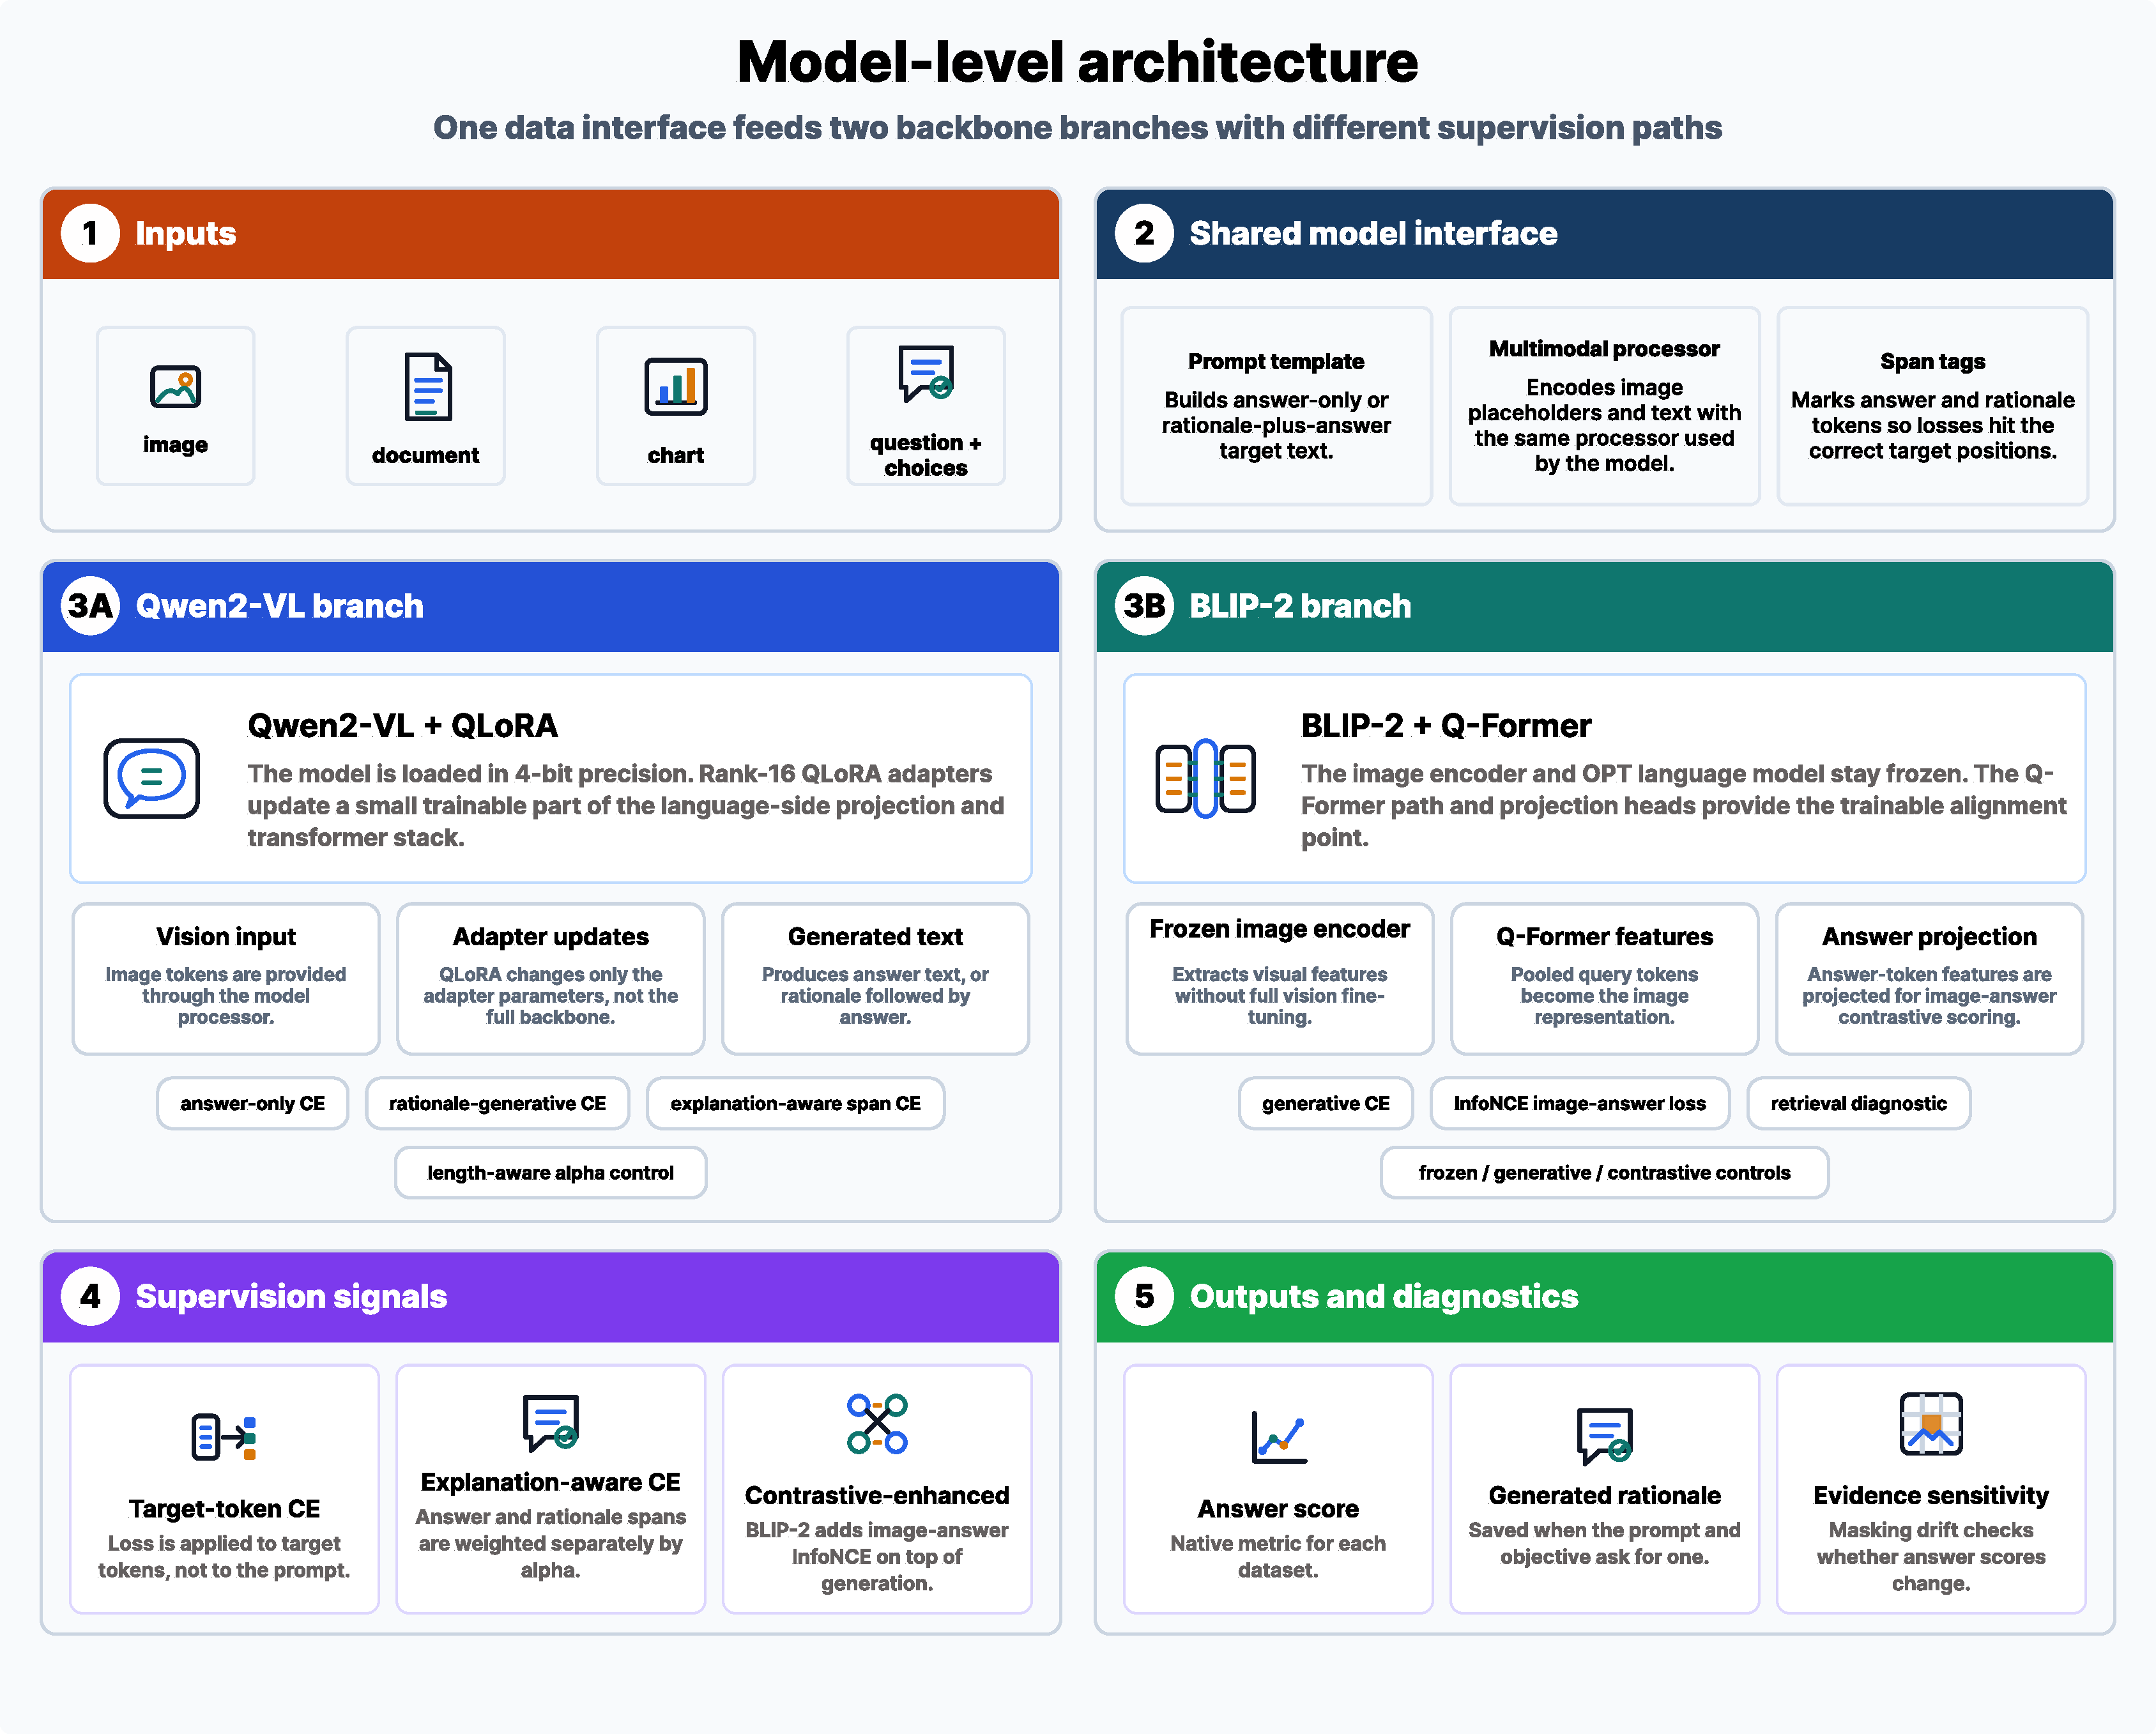
\includegraphics[height=0.74\textheight,keepaspectratio]{./Figures/icons/ModelArchitecture.pdf}}
\caption{Model-level architecture of the controlled alignment setup.
A shared multimodal interface prepares prompts, processor inputs, and supervised spans before routing the run through the Qwen2-VL QLoRA branch or the BLIP-2 Q-Former branch.
Qwen2-VL is used for answer-only, rationale-generative, and explanation-aware supervision, while BLIP-2 is used for generative and contrastive-enhanced controls.}
\label{Fig:Architecture}
\end{figure*}

\begin{equation}
    \mathcal{L} = \alpha\,\mathcal{L}_{\text{answer}} + (1-\alpha)\,\mathcal{L}_{\text{explanation}}
    \label{Eq:Loss}
\end{equation}

Here, $\mathcal{L}_{\text{answer}}$ is the masked cross-entropy loss on the answer tokens, and $\mathcal{L}_{\text{explanation}}$ is the same loss on the explanation tokens.
The coefficient $\alpha$ controls the relative weight of the answer and explanation supervision.

We use two ways of setting $\alpha$.
In fixed-alpha mode, $\alpha$ is chosen explicitly in the experiment configuration serving as an ablation control.
In length-aware mode, the effective answer weight is computed from the number of supervised answer and explanation tokens, as shown in Equation~\ref{Eq:LengthAlpha}:

\begin{equation}
    \alpha_{\text{eff}} =
    \frac{\lambda\,n_{\text{answer}}}{\lambda\,n_{\text{answer}} + n_{\text{explanation}}},
    \label{Eq:LengthAlpha}
\end{equation}
where $n_{\text{answer}}$ and $n_{\text{explanation}}$ are the answer and explanation token counts after collation, and $\lambda$ is the answer-weight multiplier.
When $\lambda=1$, the loss becomes the usual token-level cross-entropy over the full rationale-plus-answer target.
Because of this, the fixed-alpha runs are treated as the ablation, while the length-aware run is used as the natural token-weighted control.

For multiple-choice datasets, inference is done in two steps.
First, a short reasoning sequence is generated given the image and the question.
Then, given that reasoning trace, the model scores each answer option by computing the length-normalised log-likelihood of that option as a continuation of the reasoning.
Afterwards, the option with the highest score is selected as the final answer.
This avoids relying on fragile string parsing or on whether the model copied an option label correctly.
In case of open-ended datasets, the model just generates an answer string, which is evaluated using the dataset's native metric.
When a rationale is generated, it is saved for later use in the rationale quality and evidence sensitivity evaluation.

\section{Evaluation metrics}
Evaluation is divided into three parts: answer quality, rationale quality, and evidence sensitivity.
Answer quality is measured using the native metric of the benchmark, which is the primary metric reported on the leaderboard for that dataset.
We use the term ``headline metric'' to refer to this native primary metric,
not to some universal metric to be compared directly across datasets.
For ScienceQA and A-OKVQA, the headline metric is multiple-choice accuracy.
For DocVQA, it is average normalised Levenshtein similarity (ANLS), as per the benchmark convention~\cite{mathew2021docvqa}.
For ChartQA, it is relaxed accuracy for numerical answers~\cite{masry2022chartqa}.
For the VQAv2 subset, it is VQA consensus accuracy, which is computed wherever annotator answers exist~\cite{antol2015vqa,goyal2017vqav2}.

For rationale quality, we use BLEU and ROUGE-L whenever gold rationales are available~\cite{papineni2002bleu,lin2004rouge}.
These metrics do not measure faithfulness or correctness of the rationale, but they do provide a basic check on 
whether the generated explanation is lexically similar to the gold rationale, and whether it captures the same sequence of reasoning steps.

Evidence sensitivity is measured in an iterative way.
The model's answer is scored on the original image, and then scored again several times by masking out different regions of the image.
This is a general idea of occlusion sensitivity analysis~\cite{zeiler2014visualizing}, adapted to the question-answering setting.
The drift in the answer score when a region is masked out indicates how much the model's answer relies on that region as evidence.
That evidence-masking drift is shown in Equation~\ref{Eq:Drift}.
For qualitative inspection, we compare the regions with high evidence-masking drift to the content named in the generated rationale,
to see if the model is actually naming the evidence it relies on.

\begin{equation}
    \mathrm{drift}(r) = s\!\left(a \mid I\right) - s\!\left(a \mid I \setminus r\right)
    \label{Eq:Drift}
\end{equation}
where $s(a \mid I)$ is the length-normalised log-likelihood of the gold answer $a$ given image $I$, and $I \setminus r$ is the same image with region $r$ occluded.
A large positive drift says the masked region mattered.
A drift near zero says the opposite: the answer probably leaned on language priors, a shortcut, or non-visual context.
The absolute scale does not travel across datasets, since answer length, prompt family, image resolution, and task format all bend the likelihood scores.
The split it captures is the familiar one between a useful explanation and a faithful one.
It also speaks to recent hallucination and critique work, where a model happily describes or relies on visual content that simply is not there~\cite{guan2024hallusionbench,jiang2024hacl,wu2025visco,zhang2025criticv}.
That is why evidence sensitivity sits next to answer accuracy here, rather than being parked as a post-hoc example.

\section{Experimental settings and software used}

Fixed-budget protocol is applied for all the experiments, 
where every run is capped to the same number of training examples,
the same number of evaluation examples, and the same number of seeds.
For Qwen2-VL, the default setup is AdamW optimizer with a learning rate of $2 \times 10^{-4}$,
cosine decay, three percent warm-up, weight decay of 0.01, bf16 compute, and an effective batch size of 32 through gradient accumulation.
The base model is loaded with 4-bit NormalFloat (NF4) quantisation.
QLoRA adapters use rank 16 and scaling factor 32~\cite{hu2022lora,dettmers2023qlora}.
Qwen2-VL-2B-Instruct is the main backbone because it is strong enough while still being small enough to fit the available budget~\cite{wang2024qwen2vl}.
The BLIP-2 experiments use Salesforce BLIP-2 OPT-2.7B, where only Q-Former-side components are trainable, while the vision tower and the OPT language model are frozen~\cite{li2023blip2}.
Qwen2-VL-7B with the same QLoRA setting is used for the scale test.

The split, filtered example count, seed, objective, adapter configuration, and evaluation metrics are recorded for each run.
A split-and-leakage audit is performed for every run, to check the overlap between the train and evaluation identifiers.
The overlap between train and evaluation in the final artifact is zero.
The only non-standard split is DocVQA.
The loaded source provides only validation and test.
That is why the experiment run uses \texttt{validation[:80\%]} for training and \texttt{validation[80\%:]} for evaluation, with native-ID overlap checking.
That audit shows zero native-ID overlap, but it does not guarantee that the train and evaluation sets are completely disjoint in terms of visual content, because the dataset contains multiple questions per document.
For that reason, the DocVQA score is viewed as an internal adaptation result, not as a benchmark claim.

Approximate uncertainty estimates are reported for the accuracy-style headline metrics.
Since most evaluation sets are 200 examples and only a small number of seeds fit the budget,
very small gaps like 0.790 versus 0.795 are treated as observed differences rather than statistically significant ones.
Table~\ref{tab:Config} gives the default configuration used for the Qwen2-VL runs.

\begin{table}[!ht]
\centering
\caption{Default Qwen2-VL QLoRA fine-tuning configuration. BLIP-2 contrastive runs use the separately reported frozen-vision/frozen-LLM Q-Former training setup. Any run that changes these values is reported separately in the experiment ledger and in the Results section.}
\label{tab:Config}
\begin{tabular}{|l|c|}
\hline
\multicolumn{2}{|c|}{\textbf{Training Configuration}} \\ \hline
Adapter & QLoRA (4-bit NF4, rank 16, scaling 32) \\
Optimizer & AdamW ($\beta_1$=0.9, $\beta_2$=0.999) \\
Learning rate & $2 \times 10^{-4}$ (cosine, 3\% warm-up) \\
Weight decay & 0.01 \\
Effective batch size & 32 with gradient accumulation \\
Precision & bf16 compute \\
Primary seed policy & one seed per complete configuration \\ \hline
\end{tabular}
\end{table}

\section{Experiment ledger}
Before reporting the results, a summary of what each group of runs is meant to test is shown in Table~\ref{tab:ExperimentLedger}.
The key boundary is availability of gold rationales.
ScienceQA and A-OKVQA have gold rationales, meaning they support rationale-generative and explanation-aware supervision.
On the other hand, ChartQA, DocVQA, and VQAv2 do not provide the rationale target, so they are considered as answer-only fallback runs for the domain and transfer analyses.

\begin{table*}[!ht]
\centering
\caption{Main experiment ledger. The full generated ledger includes exact caps, seeds, prompt variants, alpha mode, and configuration hashes.}
\label{tab:ExperimentLedger}
\small
\renewcommand{\arraystretch}{1.15}
\begin{tabular}{|>{\raggedright\arraybackslash}p{0.20\textwidth}|>{\raggedright\arraybackslash}p{0.36\textwidth}|>{\raggedright\arraybackslash}p{0.34\textwidth}|}
\hline
\textbf{Comparison} & \textbf{Runs included} & \textbf{Use in the paper} \\ \hline
BLIP-2 objective pair & BLIP-2 OPT-2.7B on ScienceQA: generative and generative+contrastive. & Tests whether the auxiliary contrastive objective contributes anything beyond BLIP-2 generative fine-tuning. \\
ScienceQA controls & Qwen2-VL-2B on ScienceQA: answer-only, rationale+answer CE, fixed-$\alpha$ explanation-aware sweep, and length-aware control. & Separates answer supervision, rationale supervision, and alpha weighting on a gold-rationale dataset. \\
A-OKVQA controls & Qwen2-VL-2B on A-OKVQA: answer-only, rationale+answer CE, fixed-$\alpha$ explanation-aware, and length-aware control. & Repeats the rationale-supervision comparison on a second gold-rationale domain. \\
Fallback domains & Qwen2-VL-2B on ChartQA, DocVQA, and VQAv2 with answer-only fallback prompts. & Reports in-domain adaptation and transfer for datasets without gold rationales; these rows are not used as explanation-aware evidence. \\
Scale & Qwen2-VL-2B and Qwen2-VL-7B on ScienceQA with the same fixed explanation-aware QLoRA setting. & Checks whether the selected setup changes when the backbone scale increases. \\
Transfer & Qwen2-VL-2B source adapters evaluated on target-domain prompts across all datasets. & Tests cross-domain behaviour separately from the official in-domain result table. \\
Masking & Selected Qwen2-VL runs with image-region perturbation and saved visual examples. & Measures evidence sensitivity beside answer accuracy and rationale quality. \\ \hline
\end{tabular}
\end{table*}

\FloatBarrier
